\chapter{Quá trình thực tập tốt nghiệp, kết quả và đánh giá}
\section{Tóm tắt nội dung thực tập}
Với đề tài nhóm đã chọn ban đầu là Xây dựng hệ thống giám sát giao thông thời gian thực sử dụng camera, nhiệm vụ ban đầu của nhóm được định hình là phát triển tích hợp chức năng xem video vào hệ thống trang web đang tồn tại, chú trọng yếu tố thời gian thực với trọng tâm là nghiên cứu, ứng dụng streaming video và sử dụng thư viện bản đồ trên nền tảng J2EE. Tuy nhiên, sau khi trao đổi với Trung tâm quản lí và điều hành vận tải hành khách công cộng (QLĐHVTHKCC), yêu cầu được thay đổi như sau: 

\begin{itemize}
	\item Hiện thực chức năng đăng nhập và phát triển các chức năng dành cho người điều hành (tạm gọi là các chức năng giám sát).
	\item Chỉ có ngườii điều hành mới được xem các video.
	\item Hệ thống có khả năng phân tích các dữ liệu thực và đưa ra dự báo về khả năng kẹt xe.
\end{itemize}

\section{Kế hoạch công việc - Biểu đồ Gantt}
Dựa trên nội dung đã tóm tắt như trên, nhóm đã liệt kê các công việc và sắp xếp vào biểu đồ Gantt nhằm mục đích quản lí tiến độ một cách khoa học:

\begin{table}[H]
	\centering
	\begin{tabular}{|m{8cm}|c|c|}
		\hline
		Tên & Ngày bắt đầu & Ngày kết thúc\\
		\hline
		Lấy giấy giới thiệu từ khoa&
		18/03/2016&
		23/03/2016\\\hline
		Đến trạm điều hành, xác định yêu cầu hệ thống&
		24/03/2016&
		24/03/2016\\\hline
		Xác định feature list&
		25/03/2016&
		31/03/2016\\\hline
		Vẽ use-case diagram&
		31/03/2016&
		02/04/2016\\\hline
		Vẽ activity diagram&
		31/03/2016&
		02/04/2016\\ \hline
		Xin giấy phép lấy video URL&
		01/04/2016&
		07/04/2016\\ \hline
		Đọc hiểu source code cũ - Phần hiển thị bản đồ&
		02/04/2016&
		15/04/2016\\ \hline
		Học Leaflet, vẽ được bản đồ với Open Street Map, có nút bấm hiển thị video đơn giản&
		02/04/2016&
		15/04/2016\\ \hline
		Thiết kế giao diện web&
		09/04/2016&
		21/04/2016\\ \hline
		Demo: Map có icon xe bus, đã nhúng bảng điều khiển mẫu&
		22/04/2016&
		29/04/2016\\ \hline
		Phân tích, đánh giá hệ thống cũ&
		30/04/2016&
		06/05/2016\\ \hline
		Đọc hiểu source code cũ - Phần server&
		06/05/2016&
		12/05/2016\\ \hline
		Phân tích database, vẽ ERD&
		06/05/2016&
		12/05/2016\\ \hline
		Tìm hiểu cách tiếp nhận dữ liệu GPS, định vị vị trí xe bus trên bản đồ&
		06/05/2016&
		12/05/2016\\ \hline
		Demo: Lấy dữ liệu, cập nhật vị trí xe bus trên bản&
		06/05/2016&
		12/05/2016\\ \hline
		Tìm hiểu stream bằng Java&
		06/05/2016&
		20/05/2016\\ \hline
		Xử lý backend để stream&
		06/05/2016&
		20/05/2016\\ \hline
		Xây dựng công cụ sử dụng API của trạm điều hành để lấy dữ liệu camera&
		22/04/2016&
		27/05/2016\\ \hline
	\end{tabular}
	\caption{Danh sách công việc cần hoàn thành trong quá trình thực tập}
\end{table}

Biểu đồ Gantt được vẽ bằng công cụ Gantt Project:

\begin{figure}[H]
	\centering
	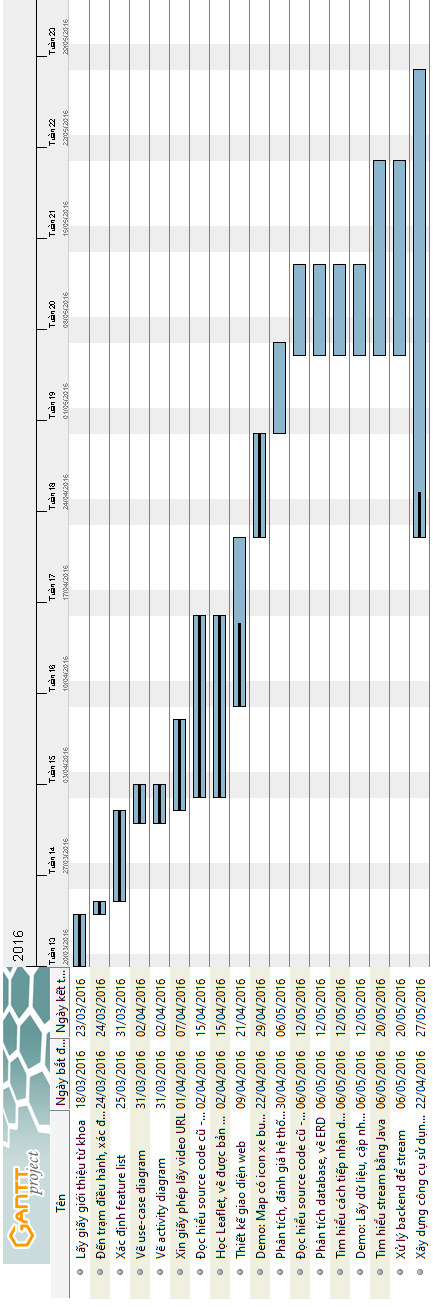
\includegraphics[scale=.6]{Graphics/gantt}
	\caption{Biểu đồ Gantt các công việc trong quá trình TTTN}
\end{figure}

\section{Kết quả thu được}
Kết quả đạt được sau 5 tháng làm việc của nhóm bao gồm những nội dung sau:
\begin{enumerate}
	\item Nắm được các kiến thức cần thiết để chuẩn bị cho việc thực hiện dự án, bao gồm những nội dung đã trình bày ở phần 3 (\textit{Xem phần 3 - Kiến thức liên quan}) và có thể sử dụng thành thạo các framework, các thư viện cũng như các kỹ thuật cần thiết (\textit{Xem Demo}).
	\item Một tài liệu đặc tả phân tich chi tiết nội dung dự án 
	(\textit{Xem phần 2 - Phân tích và đặc tả yêu cầu})
	
	\item Code dự án hiện có và một cơ sở dữ liệu tạm lưu trữ dưới dạng các file log.
	
	 Phân tích và đánh giá việc thực hiện đề tài về mặt yêu cầu cũng như cơ sở vật chất hiện có, chúng tôi có những nhận xét sau:
	
	\begin{enumerate}

		\item Về việc thực hiện đề tài:
		Đề tài yêu cầu thực hiện thêm một chức năng mới của hệ thống đã có sẵn.
		
		Do đề tài liên quan tới bên thứ 3 là Trung tâm QLĐH VTHKCC, yêu cầu của đề tài đã không được thống nhất khi chúng tôi bắt đầu tiếp cận. 

		\item Về hệ thống đang tồn tại:
		Smart BK Traffic đặt tại tên miền http://traffic.hcmut.edu.vn/ đã bắt đầu được triển khai từ trước hiện đang bao gồm các chức năng: Xem bản đồ khu vực thành phố Hồ Chí Minh và vận tốc lưu thông trung bình trên các tuyến đường.
		
		Mã nguồn được viết bằng Java, sử dụng MongoDb để lưu trữ dữ liệu về các trạng thái giao thông. Dữ liệu này thy đổi thường xuyên theo thời gian thực và được làm sạch khi bộ nhớ đầy. Client-side được viết bởi HTML5, CSS3 và javascript sử dụng thư viện Leaflet. 
		
		Thuận lợi của nhóm khi thực hiện đề tài này là mã nguồn đã được khỏi tạo trước, các công nghệ đã được lựa chọn sẵn, giao diện chính của người dùng đã được tạo ra bao gồm bản đồ và cách thức thể hiện vận tốc trên từng tuyến đường.
		
		Tuy nhiên, đó cũng là 1 khó khăn cho nhóm khi mà tiếp tục phát triển dự án trên một nền tảng cố định thiếu linh hoạt, phải dùng những công nghệ đã được ấn định trong khi nhóm chưa có cơ hội tiếp cận với mã nguồn chính thức vì lí do an ninh và bảo mật.
		
		Một vấn đề khác là dự án đang tồn tại được xây dựng mà không được tài liệu hoá, một số file mã nguồn bị thất lạc, chỉ còn lại file .class, mã nguồn không theo một pattern chính thống khiến cho việc nghiên cứu, bảo trì cũng như mở rộng gặp rất nhiều khó khăn.
		
		\item Về cơ sở dữ liệu: 
		Vì dữ liệu nhận được là frame video dưới dạng URL (Uniform Resource Locator) từ Trung tâm nên rất hạn chế và chúng tôi không thực sự biết được kết cấu dữ liệu của họ. Ngoài ra các video này chỉ có thể chạy trên trình duyệt Internet Explorer.
			
		Cơ sở vật chất, thiết bị của nhà trường hiện đang rất hạn chế nên chúng tôi chưa được tiếp xúc với dữ liệu thực mà chỉ làm việc với các file log.
		
		\item Biện pháp để khắc phục những khó khăn trên:
		
		Hiện giờ chúng tôi đang cố gắng tìm hiểu về dự án cũ kể cả về chức năng, kỹ thuật và kiến thức yêu cầu; tiếp thận thông tin, trao đổi và thống nhất yêu cầu giữa các bên; yêu cầu được cấp API để thực hiện đề tài; tạm thời trước hết nhanh chóng hiện thực các chức năng sao cho tương tác tốt với IE và sau đó tìm cách nâng cấp API có thể sử dụng trên trình duyệt khác.
			
	\end{enumerate}
	
	\item Demo
	
	\textit{Trang đăng nhập:}
	\begin{figure}[H]
		\centering
		\makebox[\textwidth]{
\includegraphics[width=\textwidth]{Graphics/login}}
		\caption{Demo đăng nhập}
	\end{figure}
	
	\textit{Xem video:}
	\begin{figure}[H]
		\centering
		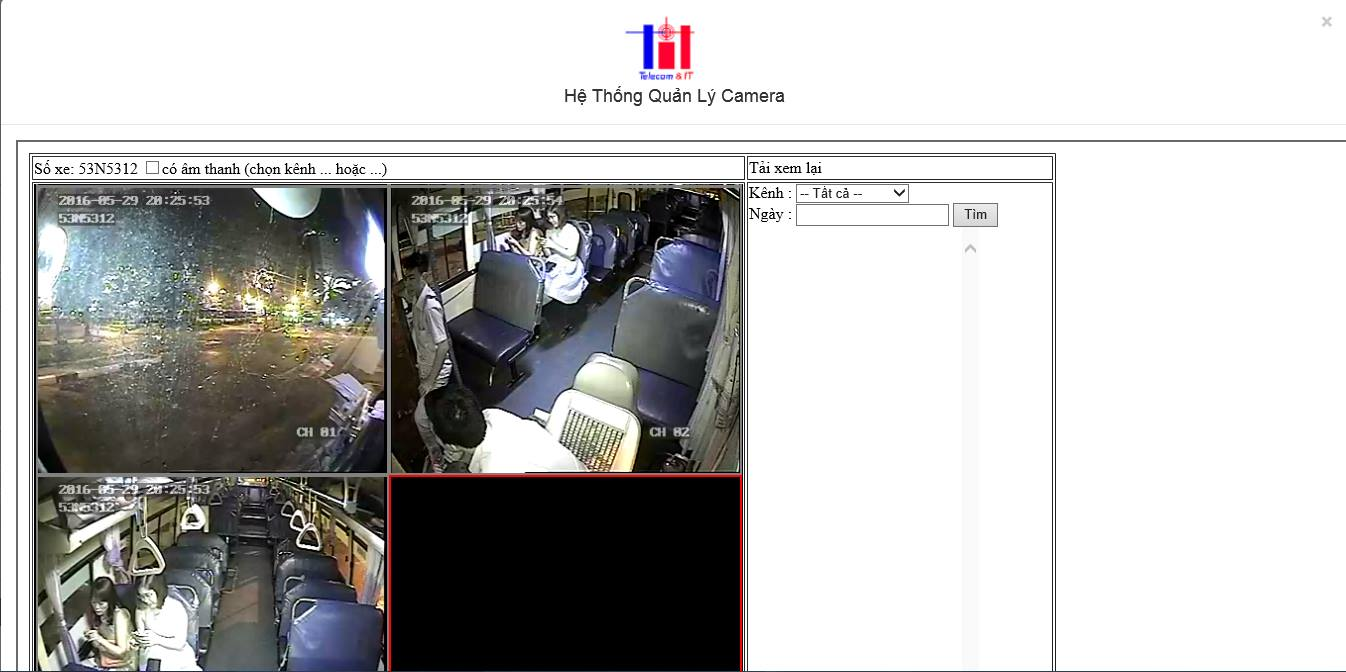
\includegraphics[width=\textwidth]{Graphics/video}
		\caption{Demo xem video trên IE}
	\end{figure}
	
	\textit{Bản đồ trên trang chính:}
	\begin{figure}[H]
		\centering
		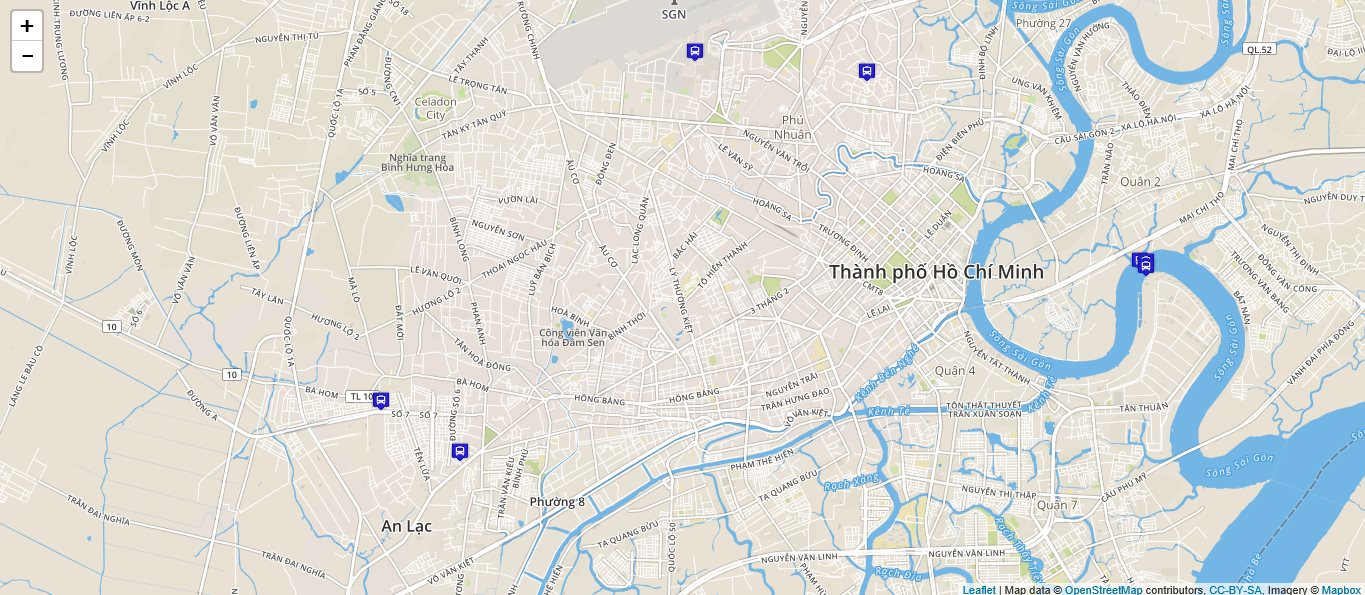
\includegraphics[width=\textwidth]{Graphics/map}
		\caption{Demo bản đồ}
	\end{figure}

	\item Báo cáo tổng kết thực tập tốt nghiệp
	
\end{enumerate}

\section{Đánh giá kết quả}

Nhóm chúng tôi đã hoàn thành hầu hết những nhiệm vụ đã đặt ra trong giai đoạn thực tập tốt nghiêp và theo đúng tiến độ (Xem phần 4.2 - Kế hoạch công việc). Tuy nhiên, một số vấn đề chưa thực sự được giải quyết, chẳng hạn như việc phân tích database và việc thử tích hợp treaming video. Nguyên do là vì hạn chế về việc tiếp cận dữ liệu và API đã nói ở trên.
